\section{\textit{Parameter Efficient Fine-Tuning}}

\textit{Fine-tuning} dari \textit{pre-trained model} terbukti efektif untuk berbagai tugas NLP \parencite{fine_tuning}. Namun, melakukan \textit{fine-tuning} pada seluruh model termasuk tidak efektif secara parameter karena akan menghasilkan model baru untuk setiap tugas yang dilatih. Apalagi dengan jumlah parameter yang mencapai jutaan bahkan miliaran, model yang dihasilkan dari \textit{fine-tuning} akan sangat tidak efisisen. Banyak penelitian yang mengajukan teknik \textit{fine-tuning} yang efisien secara parameter, yaitu \PEFT dengan hanya melakukan \textit{tuning} pada sebagian dari parameter model.

\subsection{\textit{Bottleneck Adapter}}

\textit{Bottleneck adapter} merupakan modul \textit{adapter} dengan menggunakan arsitektur \textit{bottleneck} \parencite{adapter_houlsby}. Konsep \textit{bottleneck adapter} diajukan sebagai alternatif dari \textit{fine-tuning}, dengan tiga properti utama, yaitu kinerja yang baik, pelatihan yang sekuensial (tidak perlu akses secara simultan terhadap keseluruhan \textit{dataset}), dan hanya menambahkan sebagain kecil parameter untuk setiap tugas \parencite{adapter_houlsby}. Strategi \textit{fine-tuning} dengan \textit{adapter} dilakukan dengan memasukkan \textit{layer} tambahan pada arsitektur \textit{Transformer} seperti yang bisa dilihat pada gambar \ref{fig:adapters_houlsby_arch}. Seperti yang telah dibahas pada subbab \ref{sec:transformer}, setiap \textit{layer} pada \textit{Transformer} mempunyai dua \textit{sub-layer}, yaitu \textit{multi-head attention} dan \textit{feed-forward}. Metode \textit{bottleneck adapter} ini akan menambahkan modul \textit{adapter} ke setiap \textit{sub-layer} pada \textit{Transformer} tersebut \parencite{adapter_houlsby}.

\begin{figure}[h]
    \vspace{0.25cm}
    \centering
    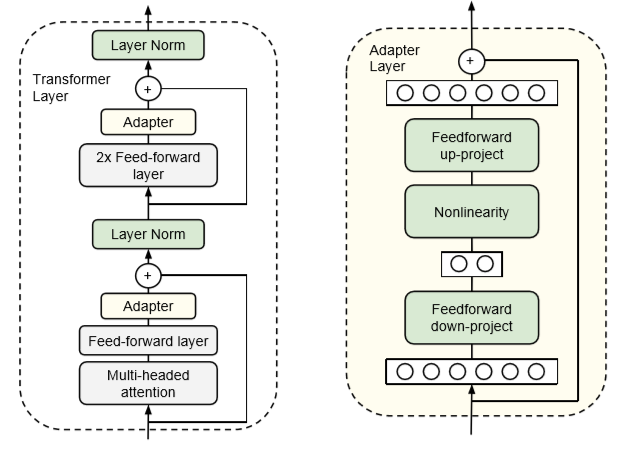
\includegraphics[width=\textwidth]{chapter-2/adapter_houlsby_arch.png}
    \caption{Arsitektur dari \textit{Bottleneck Adapter} oleh \citeauthor{adapter_houlsby} \parencite{adapter_houlsby}}
    \label{fig:adapters_houlsby_arch}
\end{figure}

Arsitektur \textit{bottleneck} dari modul \textit{adapter} diajukan untuk membatasi jumlah dari parameter \parencite{adapter_houlsby}. Berdasarkan gambar \ref{fig:adapters_houlsby_arch}, \textit{adapter} melakukan proyeksi dari dimensi asli $d$ ke dimensi yang lebih kecil $m$, lalu dilanjutkan dengan fungsi nonlinear, dan dilakukan proyeksi kembali dari dimensi $m$ ke dimensi asli $d$. Sehingga, total parameter yang ditambahkan untuk setiap \textit{layer} adalah $2md$ yang berasal dari bobot pada kedua proyeksi ditambah dengan $m+d$ yang merupakan biasnya. Pada penggunaannya, dengan memakai nilai $m << d$, parameter yang digunakan adalah sekitar $0.5-8\%$ dari parameter asli model \parencite{adapter_houlsby}.

\begin{equation}
    reduction\_factor = \frac{d_{hidden}}{d_{bottleneck}}
    \label{eq:reduction_factor}
\end{equation}

Parameter yang digunakan dibatasi dengan menggunakan $reduction\_factor$ \parencite{adapterhub}. Nilai dari $reduction\_factor$ tersebut didapat dari rasio antara dimensi asli dengan dimensi yang lebih kecil bisa dilihat pada rumus \ref{eq:reduction_factor} \parencite{adapterhub}. Nilai $d_{hidden}$ merupakan nilai dari dimensi asli $d$. Sedangkan, nilai $d_{bottleneck}$ merupakan dimensi dari \textit{bottleneck} yang lebih kecil dari dimensi aslinya.

Penggunaan \textit{adapter} tidak hanya dengan menambahkannya pada setiap \textit{sub-layer Transformer}. Terdapat beberapa konfigurasi yang bisa digunakan. Salah satunya adalah seperti pada gambar \ref{fig:adapters_houlsby_arch} oleh \parencite{adapter_houlsby} dengan menambahkan modul \textit{adapter} pada kedua \textit{sub-layer} (\textit{multi-head attention} dan \textit{feed-forward}). \citeauthor{adapter_pfeiffer} menggunakan \textit{adapter} hanya pada \textit{sub-layer feed-forward}. Sedangkan, \citeauthor{uvpl} menggunakan \textit{adapter} secara paralel pada \textit{layer transformer}.

\begin{table}[h]
    \vspace{0.25cm}
    \centering
    \caption{Hasil evaluasi \textit{Adapter} konfigurasi \citeauthor{adapter_houlsby} pada GLUE \parencite{adapter_houlsby}}
    \label{table:adapter_houlsby_result}
    \resizebox{\textwidth}{!}{
    \begin{tabular}{l|p{2cm}|p{2cm}|ccccccccc|c}
        \toprule
        & Total num params & Trained params / task & CoLA & SST & MRPC & STS-B & QQP & MNLI$_m$ & MNLI$_{mm}$ & QNLI & RTE & Total \\
        \midrule
        BERT$_{LARGE}$ & $9.0\times$ & $100\%$ & $60.5$ & $94.9$ & $89.3$ & $87.6$ & $72.1$ & $86.7$ & $85.9$ & $91.1$ & $70.1$ & $80.4$ \\
        Adapters (8-256) & $1.3\times$ & $3.6\%$ & $59.5$ & $94.0$ & $89.5$ & $86.9$ & $71.8$ & $84.9$ & $85.1$ & $90.7$ & $71.5$ & $80.0$ \\
        Adapters (64) & $1.2\times$ & $2.1\%$ & $56.9$ & $94.2$ & $89.6$ & $87.3$ & $71.8$ & $85.3$ & $84.6$ & $91.4$ & $68.8$ & $79.6$ \\
        \bottomrule
    \end{tabular}}
\end{table}

Tabel \ref{table:adapter_houlsby_result} menunjukkan hasil evaluasi dari \textit{Adapter} dengan \textit{baseline} yang menggunakan \textit{fine-tuning} pada kakas evaluasi GLUE. \textit{Adapter} berhasil mendapatkan hasil rata-rata dengan nilai $80.0$, dibandingkan dengan \textit{fine-tuning} yang mendapatkan nilai $80.4$. Selain itu, untuk ukuran dari \textit{adapter} yang tetap yaitu dengan ukuran 64, mendapatkan hasil dengan nilai $79.6$. \textit{Adapter} mampu menyaingi kinerja \textit{fine-tuning} dengan hanya menggunakan $3.6\%$ parameter.

\subsection{\textit{Prefix-Tuning}}

\textit{Prefix-Tuning} merupakan salah satu metode PEFT yang menjadi alternatif dari metode \textit{fine-tuning} yang menggunakan vektor kontinu (disebut dengan \textit{prefix}) \parencite{prefix_tuning}. Metode ini mengambil inspirasi dari \textit{prompting}, memperbolehkan token-token berikutnya untuk memerhatikan \textit{prefix} tersebut seolah-seolah \textit{prefix} tersebut adalah \textit{virtual token} \parencite{prompt_tuning}. Mirip dengan \textit{Adapter}, \textit{prefix-tuning} hanya perlu menyimpan sedikit parameter tambahan untuk suatu tugas dengan melakukan \textit{freeze} pada parameter asli model dan hanya mengubah parameter dari \textit{prefix} tersebut.

\begin{figure}[h]
    \vspace{0.25cm}
    \centering
    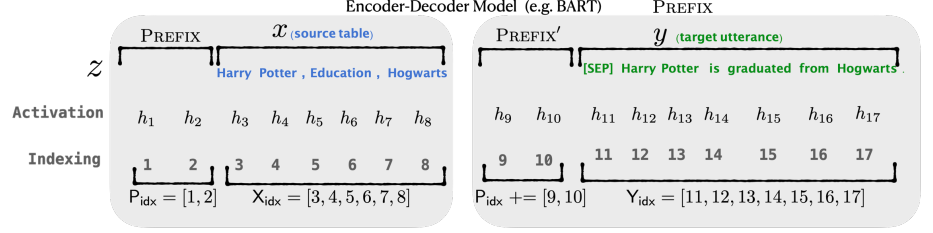
\includegraphics[width=\textwidth]{chapter-2/prefix_tuning_example.png}
    \caption{Contoh \textit{Prefix-Tuning} pada model \textit{encoder decoder} \parencite{prefix_tuning}}
    \label{fig:prefix_tuning_example}
\end{figure}

Dengan intuisi yang didapatkan dari penggunaan \textit{prompting}, penambahan konteks dapat mengarahkan model tanpa mengubah parameter \parencite{prefix_tuning}. \textit{Prefix-Tuning} menambahkan \textit{prefix} pada kedua \textit{encoder} dan \textit{decoder} untuk mendapatkan $z = [PREFIX;x;PREFIX';y]$ seperti yang bisa dilihat pada gambar \ref{fig:prefix_tuning_example}. $P_{idx}$ merupakan indeks dari \textit{prefix} tersebut. Matriks yang bisa dilatih, diinisialisasi sebagai matriks $P_\theta$ dengan $\theta$ sebagai parameternya. Dimensi dari matriks $P_\theta$ adalah panjang dari $P_{idx}$ dikalikan dengan besar dimensi \textit{activation layer}-nya yaitu $h$. Secara langsung melakukan optimisasi terhadap $P_\theta$ itu tidak stabil dan menghasilkan penurunan terhadap kinerja \parencite{prefix_tuning}. Sehingga, matriks $P_\theta$ diperamaterisasi sebagai $P_\theta = MLP_\theta(P'_\theta)$ dengan matriks dimensi lebih kecil ($P'_\theta$) dimasukkan ke dalam \textit{feed forward} ($MLP_\theta$).

\begin{figure}[h]
    \vspace{0.25cm}
    \centering
    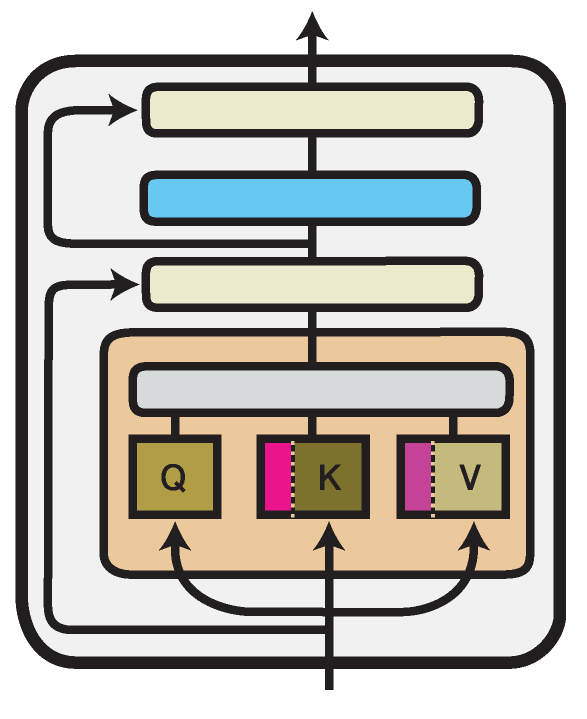
\includegraphics[height=0.4\textwidth]{chapter-2/prefix_tuning_arch.png}
    \caption{Arsitektur \textit{Prefix-Tuning} \parencite{prefix_tuning}}
    \label{fig:prefix_tuning_arch}
\end{figure}

Pada gambar \ref{fig:prefix_tuning_arch} ditunjukkan arsitektur dari \textit{Prefix-Tuning} dengan menambahkan \textit{prefix} pada \textit{multi-headattention layer}. \textit{Prefix} ditambahkan pada bagian \textit{key} dan \textit{value} pada \textit{attention head}, menjadi $P^K$ dan $P^V$. Sehingga, rumus \ref{eq:attention} akan menggunakan $[P^K, K]$ dan $[P^V, V]$ menjadi $Attention(Q, [P^K, K], [P^V, V])$ \parencite{adapterhub}. Selain itu, panjang dari \textit{prefix} dapat divariasikan berdasarkan pada nilai \textit{prefix length}-nya.

\begin{table}[h]
    \vspace{0.25cm}
    \centering
    \caption{Hasil evaluasi \textit{Prefix-Tuning} pada tugas \textit{summarization} XSUM \parencite{prefix_tuning}}
    \label{table:prefix_tuning_result}
    \begin{tabular}{lccc}
        \toprule
        Method & R-1 & R-2 & R-L \\
        \midrule
        FINE-TUNE & $45.14$ & $22.27$ & $37.25$ \\
        PREFIX($2\%$) & $43.80$ & $20.93$ & $36.05$ \\
        PREFIX($0.1\%$) & $42.92$ & $20.03$ & $35.05$ \\
        \bottomrule
    \end{tabular}
\end{table}

Pada penelitian yang dilakukan oleh \citeauthor{prefix_tuning}, terdapat dua tugas yang dievaluasi yaitu \textit{table-to-text generation} dan \textit{summarization}. Seperti yang bisa dilihat pada tabel \ref{table:prefix_tuning_result}, dengan hanya $2\%$ parameter dibanding parameter aslinya, \textit{Prefix-Tuning} berhasil mendapatkan kinerja yang sedikit lebih buruk dibanding \textit{fine-tuning} ($36.05$ dibanding $37.25$ pada R-L) \parencite{prefix_tuning}. Hasil ini sedikit berbeda dibanding pada tugas \textit{table-to-text generation} yang mendapatkan hasil yang menyaingi \textit{fine-tuning}. Perbedaan antara kedua tugas tersebut adalah bahwa masukan dari artikel pada XSUM lebih banyak sekitar 17 kali dibanding pada \textit{dataset table-to-text}, serta tugas \textit{summarization} lebih kompleks dibanding \textit{table-to-text generation} karena perlu pemahaman terhadap tulisandan mengidentifikasi topik penting dari sebuah artikel \parencite{prefix_tuning}.

\subsection{\textit{Low Rank Adaptation} (LoRA)}

\textit{Low Rank Adaptation} atau biasa disebut sebagai LoRA merupakan salah satu metode PEFT. Berbeda dengan metode PEFT yang dibahas sebelumnya pada subbab sebelumnya, penambahan \textit{adapter} seperti yang dilakukan oleh \citeauthor{adapter_houlsby} akan menambahkan waktu inferensi \parencite{lora}. Selain itu, melakukan optimisasi pada input dengan menggunakan "\textit{prompt}" seperti yang dilakukan oleh \citeauthor{prefix_tuning} itu sulit untuk dioptimasi dan kinerjanya tidak selalu meningkat \parencite{lora}. Dengan menambahkan panjang dari sekuens masukan akan mengurangi sekuens yang seharusnya bisa digunakan untuk suatu tugas \parencite{lora}. Sehingga, metode tersebut sering kali gagal dalam menyaingi kinerja dari \textit{fine-tuning}, bahkan memerlukan adanya \textit{tradeoff} antara kinerja dengan efisiensi \parencite{lora}.

\begin{figure}[h]
    \vspace{0.25cm}
    \centering
    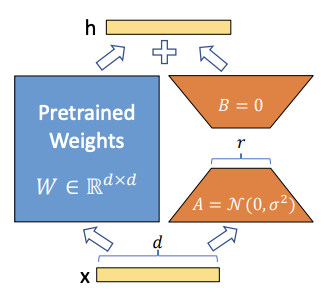
\includegraphics[width=0.6\textwidth]{chapter-2/lora.png}
    \caption{Arsitektur LoRA \parencite{lora}}
    \label{fig:lora_arch}
\end{figure}

LoRA menggunakan pendekatan bahwa parameter dari model yang dilatih sebenarnya berada pada dimensi instrinsik yang rendah dan masih dapat belajar secara efisien pada dimensi yang lebih rendah tersebut \parencite{lora}. Untuk matriks beban $W_0$ dari sebuah \textit{pre-trained model} dengan dimensi $d\times{k}$, dekomposisi dengan \textit{rank} $r$ (\textit{low-rank decomposition}) dapat direpresentasikan sebagai $W_0 + \Delta{W} = W_0 + BA$, dengan dimensi $B$ adalah $d\times{r}$ dan dimensi $A$ adalah $r\times{k}$, dan \textit{rank} $r << min(d,k)$ \parencite{lora}. Bisa dilihat pada gambar \ref{fig:lora_arch}, LoRA menggunakan matriks dengan rank yang lebih rendah pada matriks $A$ dan matriks $B$. Matriks $A$ diinisialisasi dengan gaussian, sedangkan matriks $B$ diinisialisasi dengan 0. Sehingga, pada awal pelatihan nilai dari $\Delta{W}=BA$ adalah 0. Ketika proses pelatihan, matriks beban $W_0$ dilakukan \textit{freeze}, sedangkan mariks $B$ dan $A$ adalah parameter yang dilatih \parencite{lora}.

\begin{table}[ht]
    \vspace{0.25cm}
    \centering
    \caption{Hasil evaluasi LoRA dengan model GPT-3 \parencite{lora}}
    \label{table:lora_result}
    \resizebox{ \textwidth }{!}{
        \begin{tabular}{l|p{2.5cm}|ccccc}
            \toprule
            Method & \# Trainable Parameters & WikiSQL & MNLI-m & \multicolumn{3}{c}{SAMSum} \\
             & & \textbf{Acc. (\%)} & \textbf{Acc. (\%)} & \textbf{R1} & \textbf{R2} & \textbf{RL} \\
            \midrule
            FT & 175,255.8M & \textbf{73.8} & 89.5 & 52.0 & 28.0 & 44.5 \\
            BitFit & 14.2M & 71.3 & 91.0 & 51.3 & 27.4 & 44.5 \\
            PreEmbed & 3.2M & 63.1 & 88.6 & 48.4 & 24.2 & 40.5 \\
            PreLayer & 20.2M & 70.1 & 89.5 & 50.8 & 27.3 & 44.5 \\
            Adapter\textsubscript{H}  & 7.1M & 71.9 & 89.8 & 53.0 & 28.9 & 44.9 \\
            Adapter\textsubscript{L}  & 40.1M & 73.2 & \textbf{91.5} & 53.2 & 29.0 & 45.1 \\
            LoRA  & 4.7M & 73.4 & 91.7 & \textbf{53.8} & \textbf{29.8} & \textbf{45.9} \\
            LoRA  & 37.7M & \textbf{74.0} & 91.6 & 53.4 & 29.2 & 45.1 \\
            \bottomrule
        \end{tabular}
    }
\end{table}

Hasil evaluasi LoRA pada beberapa tugas evaluasi dapat dilihat pada tabel \ref{table:lora_result}. LoRA mampu menyaingi atau bahkan melampaui kinerja \textit{fine-tuning} pada ketiga tugas evaluasi tersebut. Selain itu, dari dibandingkan metode PEFT yang lain, LoRA menghasilkan skalabilitas dan kinerja yang lebih baik \parencite{lora}.
